\vspace{-4mm}

\section{Empirical Results on PreTrained DNNs}
\label{sxn:emp}

\paragraph{VGG and VGG BN Models}

We start by looking at the VGG class of models, including VGG11, VGG13, VGG16, and VGG19, and their counterparts with Batch Normalization, 
VGG11\_BN, VGG13\_BN, VGG16\_BN and VGG19\_BN.  Figure~\ref{fig:vgg}

\begin{table}[t]
\small
\begin{center}
\begin{tabular}{|p{1in}|c|c|c|c|c|c|c|}
\hline
Architecture 
 & Model &Top1 
 & Top5 & $L$ & $N_{\alpha}$ & $\hat{\alpha}$ & $\hat{\alpha}*$ \\
\hline
VGG11 & VGG11 &  & & & & \\
  & VGG11 BN & & \\
\hline
VGG13 & VGG13 & & \\
  & VGG13 BN & &\\
\hline
VGG16 & VGG16 & & \\
  & VGG16 BN & & \\
\hline
VGG19 & VGG19 & \\
  & VGG19 BN & & \\
\hline
\end{tabular}
\end{center}
\caption{VGG Architectures and DNN Models}
\label{table:models}
\end{table}


\begin{figure}[!htb]
 \centering
   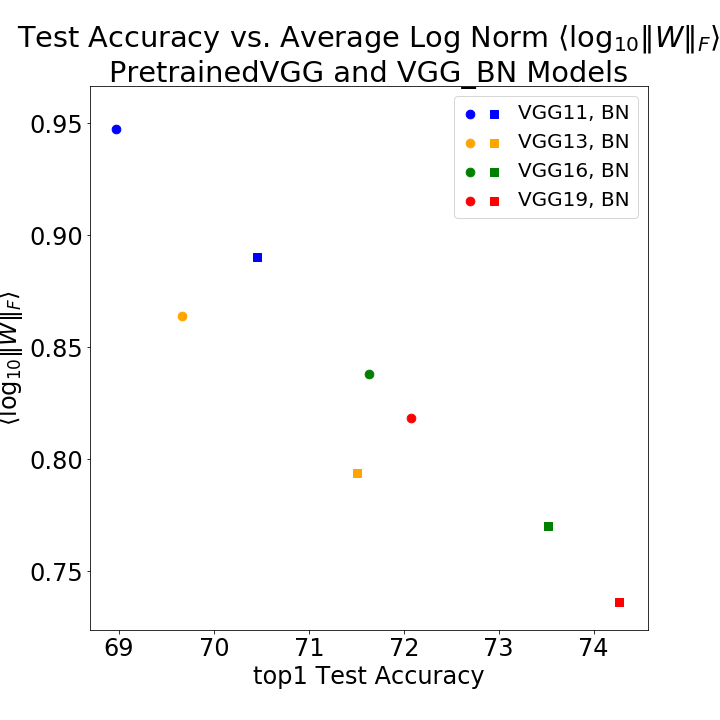
\includegraphics[scale=0.40]{img/vgg-lognorms.png}
   \caption{
Pretrained VGG and VGG BN Architectures and DNNs.  Test Accuracy and average log norm $\hat{\alpha*}$ for
 VGG11 vs VGG11\_BN ({\color{blue}{blue}}),
VGG13 vs VGG13\_BN ({\color{orange}{orange}}),
VGG16 vs VGG16\_BN ({\color{green}{green}}),  and
VGG19 vs VGG19\_BN ({\color{red}{red}}). 
Note that $\hat{\alpha}*$ does not include the last layer, connecting the model to the labels.
}
  \label{fig:vgg}
\end{figure}


\paragraph{ResNet Models}

\begin{figure}[!htb]
 \centering
   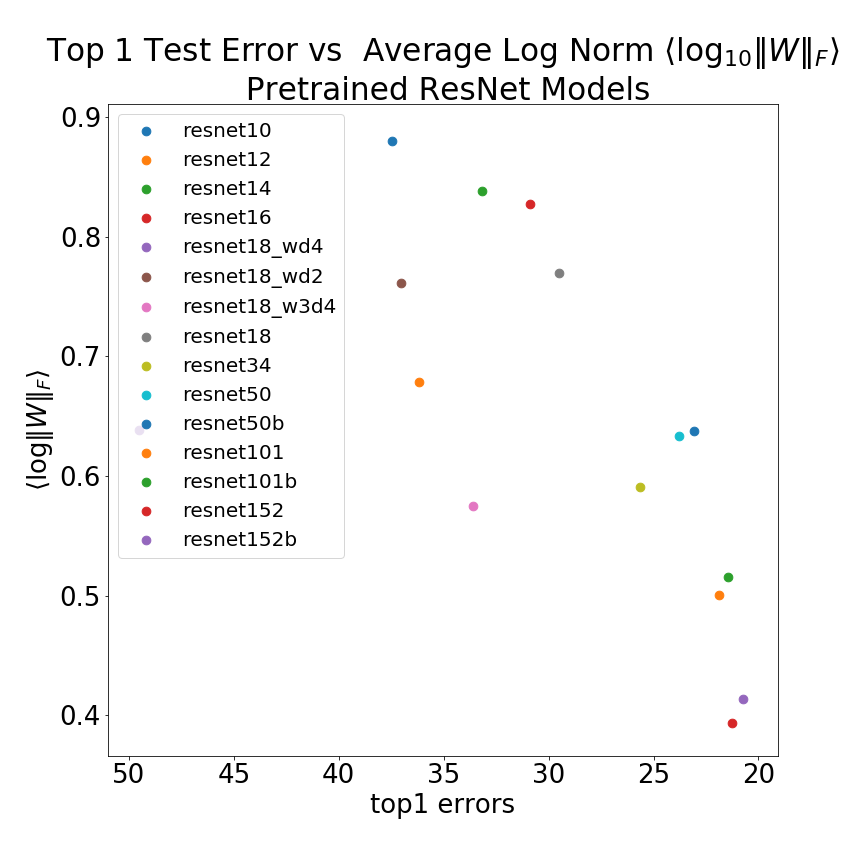
\includegraphics[scale=0.40]{img/ResNet_top1-lognorms.png}
   \caption{
Pretrained ResNet models.
}
  \label{fig:resnet}
\end{figure}



\paragraph{More PreTrained Models}

More Pretrained Models


\begin{table}[t]
\small
\begin{center}
\begin{tabular}{|p{1in}|c|c|c|c|c|c|c|}
\hline
Architecture 
 & Model
 & Test Accuracy \\
\hline
ResNet (larger) & & \\
\hline
ResNet (extended) & & \\
\hline
ResNet (b) & & \\
\hline
\end{tabular}
\end{center}
\caption{ResNet Architectures and DNN Models}
\label{table:models}
\end{table}




\begin{table}[t]
\small
\begin{center}
\begin{tabular}{|p{1in}|c|c|c|c|c|c|c|}
\hline
Architecture 
 & Model
 & Test Accuracy \\
\hline
GoogLeNet & & \\
\hline
ResNeXt & & \\
\hline
SqueezeNet & & \\
\hline
\end{tabular}
\end{center}
\caption{Other Models}
\label{table:models}
\end{table}




\begin{figure}[!htb]
    \centering
    \subfigure[DenseNet] {
        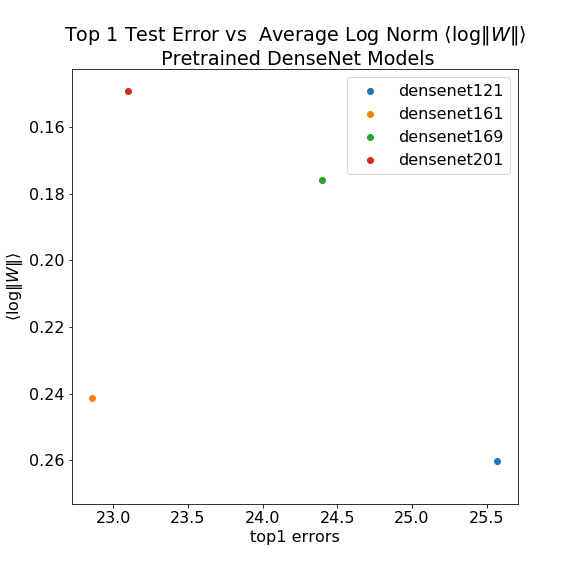
\includegraphics[scale=0.3]{img/DenseNet_top1-lognorms.png} 
        \label{fig:densenet}
    }
    \subfigure[SeResNet]{
        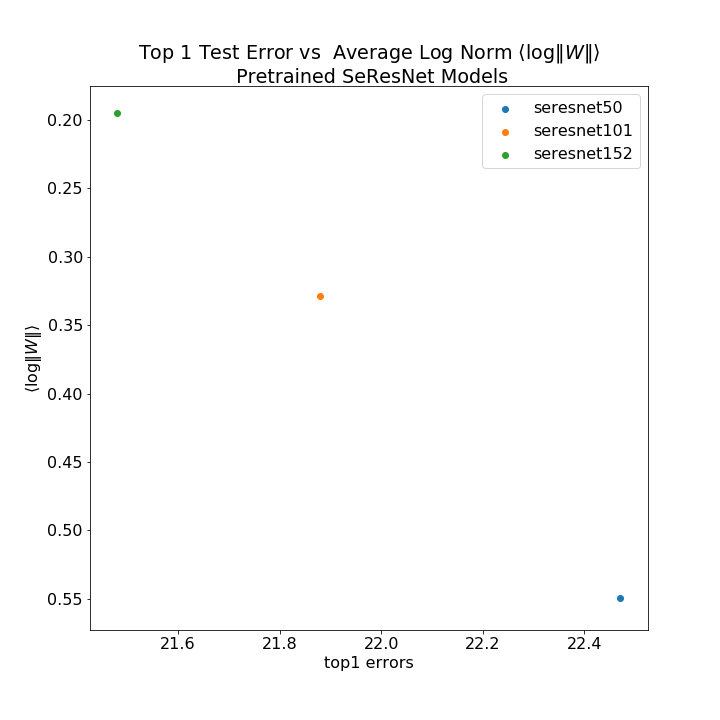
\includegraphics[scale=0.3]{img/SeResNet_top1-lognorms.png} 
        \label{fig:seresnet}
    }
        \caption{Densenet, SeResNet, and SqueezeNet Models}
    \label{fig:other2}
\end{figure}





